\documentclass[aspectratio=169,11pt]{beamer}

\usepackage{graphicx}
\usepackage{tikz}
\usetikzlibrary{positioning,arrows.meta}
\usepackage{xcolor}
\usepackage{booktabs}
\usepackage{tabularx}
\usepackage{array}
\usepackage{ragged2e}

\definecolor{GEUBlue}{RGB}{20,55,105}
\definecolor{GEULightBlue}{RGB}{238,244,251}
\definecolor{GEUGrey}{RGB}{90,90,90}
\definecolor{GEULightGrey}{RGB}{245,246,248}

\usetheme{default}
\setbeamertemplate{navigation symbols}{}
\setbeamertemplate{blocks}[rounded][shadow=false]
\setbeamercolor{normal text}{fg=black,bg=white}
\setbeamercolor{frametitle}{fg=GEUBlue}
\setbeamercolor{structure}{fg=GEUBlue}
\setbeamercolor{block title}{fg=GEUBlue,bg=GEULightBlue}
\setbeamercolor{block body}{fg=black,bg=GEULightBlue}
\setbeamerfont{frametitle}{size=\Large,series=\bfseries}

% Replace with the actual logo filename
\newcommand{\GEULogo}{graphicera_logo.png}

% Header and footer
\setbeamertemplate{headline}{%
  \begin{tikzpicture}[remember picture,overlay]
    \node[anchor=north east,xshift=-0.30cm,yshift=-0.12cm]
      at (current page.north east)
      {\includegraphics[height=0.62cm]{\GEULogo}};
  \end{tikzpicture}
  \vspace{0.72cm}
}
\setbeamertemplate{frametitle}{%
  \vspace{0.03cm}
  \insertframetitle\par
  \vspace{0.04cm}
  \textcolor{GEUBlue}{\rule{\textwidth}{0.9pt}}
  \vspace{0.03cm}
}
\setbeamertemplate{footline}{%
  \leavevmode
  \hbox{%
  \begin{beamercolorbox}[wd=.82\paperwidth,ht=0.32cm,dp=0.10cm,leftskip=.3cm]{author in head/foot}
    \tiny Department of Computer Science \& Engineering | Graphic Era (Deemed to be University)
  \end{beamercolorbox}%
  \begin{beamercolorbox}[wd=.18\paperwidth,ht=0.32cm,dp=0.10cm,rightskip=.3cm]{date in head/foot}
    \hfill\tiny\insertframenumber/\inserttotalframenumber
  \end{beamercolorbox}}
}

\newcommand{\smallnote}[1]{\vspace{0.08cm}{\scriptsize\color{GEUGrey}#1}}

\title{\textbf{Project-Based Learning}\\[2mm]\large Phase-I Evaluation}
\author{\textbf{EcoGraph -- Graph Based Algorithmic Waste Management}\\Team ID: DSCPP-III-2026-T186}
\institute{Department of Computer Science \& Engineering\\Graphic Era (Deemed to be University), Dehradun}
\date{Academic Session 2026--27}

\begin{document}

% 1
\begin{frame}[plain]
\begin{tikzpicture}[remember picture,overlay]
\draw[GEUBlue,line width=3pt] (current page.north west) -- (current page.north east);
\node[anchor=north east,xshift=-0.45cm,yshift=-0.35cm] at (current page.north east)
{\includegraphics[height=1.0cm]{\GEULogo}};
\node[align=center,text width=.84\paperwidth] at ([yshift=.25cm]current page.center)
{{\color{GEUBlue}\fontsize{26}{30}\selectfont\bfseries PROJECT-BASED LEARNING}\\[3mm]
 {\fontsize{18}{22}\selectfont PHASE-I EVALUATION}\\[7mm]
 {\color{GEUGrey}\large\bfseries EcoGraph -- Graph Based\\Algorithmic Waste Management}\\[3mm]
 {\color{GEUBlue}\normalsize Team ID: DSCPP-III-2026-T186}};
\node[align=center,anchor=south,yshift=.42cm] at (current page.south)
{\bfseries Department of Computer Science \& Engineering\\
Graphic Era (Deemed to be University), Dehradun\\[-1mm]
\scriptsize Academic Session 2026--27};
\end{tikzpicture}
\end{frame}

% 2
\begin{frame}{Team \& Mentor Details}
\begin{columns}[T,totalwidth=\textwidth]
\column{.48\textwidth}
\begin{block}{Team Information}
\begin{tabular}{@{}ll@{}}
\textbf{Team ID:} & DSCPP-III-2026-T186\\
\textbf{Semester:} & 3rd\\
\textbf{Section:} & A / D / H\\
\textbf{Domain:} & Graph Algorithms (C++)
\end{tabular}
\end{block}
\column{.48\textwidth}
\begin{block}{Team Members}
1.\quad Tejas Jain -- 2028228 (SEC-A)\\
2.\quad Yash Nigam -- 2028289 (SEC-H)\\
3.\quad Apoorv Negi -- 2027640 (SEC-D)
\end{block}
\end{columns}
\vspace{2mm}
\begin{block}{Mentor}
Navneet Rajput
\hfill
\textbf{Interactions completed:} \underline{\hspace{12mm}}
\end{block}
\end{frame}

% 3
\begin{frame}{Problem Statement \& Motivation}
\small
\begin{block}{Problem Statement}
Municipal waste routes are static, ignoring the real shortest path between homes, bins, and the depot -- wasting fuel and time. Hazardous waste (medical, chemical) is handled like ordinary waste despite needing immediate, restricted-zone pickup, and fixed schedules over- or under-service locations with different fill rates.
\end{block}
\vspace{1mm}
\begin{columns}[T,totalwidth=\textwidth]
\column{.48\textwidth}
\textbf{\color{GEUBlue}Motivation}
\begin{itemize}\itemsep1pt
\item Fixed routes ignore real shortest paths in the city graph
\item Hazardous waste in normal queues risks exposure delays
\item Uniform schedules waste trips or under-serve fast bins
\end{itemize}
\column{.48\textwidth}
\textbf{\color{GEUBlue}Target Users / Stakeholders}
\begin{itemize}\itemsep1pt
\item Municipal waste collection departments
\item Residents and commercial establishments served
\item Public health -- faster hazardous waste clearance
\end{itemize}
\end{columns}
\end{frame}

% 4
\begin{frame}{Objectives}
\small
\textbf{\color{GEUBlue}Project Objectives}
\vspace{1mm}
\begin{enumerate}\itemsep3pt
\item Model the city as a weighted graph (depot, homes, junctions, bins) tagged by zone type.
\item Compute optimal routes using Dijkstra's algorithm, with selectable Priority and FIFO strategies.
\item Detect and immediately dispatch hazardous waste via a zone-constrained shortest path avoiding residential/commercial areas.
\item Dynamically schedule collection frequency per location based on its fill-rate.
\item Expose all functionality through a REST API with live route animation on the frontend.
\end{enumerate}
\vfill
\begin{center}
\colorbox{GEULightBlue}{\parbox{.82\textwidth}{\centering
\textbf{Key Objective:} A persistent C++ backend that computes correct, zone-aware, fill-rate-driven collection routes and serves them as JSON to an animated web frontend.}}
\end{center}
\end{frame}

% 5
\begin{frame}{Proposed Solution}
\footnotesize
\begin{columns}[T,totalwidth=\textwidth]
\column{.48\textwidth}
\textbf{\color{GEUBlue}Proposed Approach}
\begin{enumerate}\itemsep2pt
\item City layout loaded from JSON config at startup
\item Dijkstra's algorithm (plain + zone-constrained) as the core routing engine
\item Priority/FIFO route builders + fill-rate scheduler
\item In-memory graph state (\texttt{unordered\_map})
\item REST API (JSON) + Cytoscape.js animation
\end{enumerate}
\column{.48\textwidth}
\textbf{\color{GEUBlue}Key Features}
\begin{itemize}\itemsep2pt
\item Graph-based city model with zone tagging
\item Shortest-path routing (Priority / FIFO toggle)
\item Rule-based waste classification (keywords)
\item Hazardous waste: immediate, constrained routing
\item Dynamic collection frequency from fill-rate
\end{itemize}
\end{columns}
\vfill
\smallnote{A single persistent C++ server owns the graph, performs routing/classification/scheduling in-process, serves JSON to the JS frontend.}
\end{frame}

% 6
\begin{frame}{Integration of PBL Course Concepts}
\scriptsize
\begin{center}
\renewcommand{\arraystretch}{1.25}
\begin{tabularx}{.96\textwidth}{@{}>{\bfseries}p{3.0cm}X p{2.7cm}@{}}
\toprule
Course & Concepts Applied & Project Module\\
\midrule
Data Structures in C & Graph (adjacency list), Queue (FIFO), Priority queue / min-heap, Hash map (\texttt{unordered\_map}) & Graph model, Scheduler, Router\\
OOPs with C++ & Classes for \texttt{Graph}, \texttt{Node}, \texttt{Edge}, \texttt{Scheduler}, \texttt{Router}; STL containers; encapsulated domain layer & Backend domain layer (\texttt{graph.hpp}, \texttt{scheduler.hpp}, \texttt{router.hpp})\\
\bottomrule
\end{tabularx}
\end{center}
\vfill
\begin{center}
\colorbox{GEULightBlue}{\parbox{.86\textwidth}{\centering
\textbf{Integration:} The city graph (DSA: adjacency list + hashing) is implemented as C++ classes (OOP: encapsulation, STL) exposing Dijkstra, constrained Dijkstra, FIFO/priority-queue-based routing, and scheduling as one cohesive backend.}}
\end{center}
\end{frame}

% 7
\begin{frame}{System Architecture / Workflow}
\begin{center}
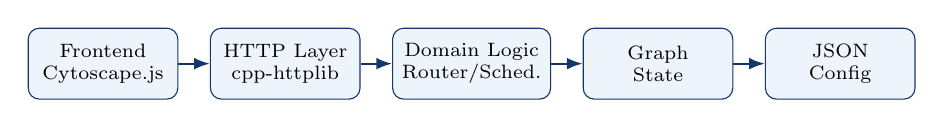
\begin{tikzpicture}[
node distance=4mm,
box/.style={rectangle,rounded corners,draw=GEUBlue,fill=GEULightBlue,
minimum width=1.9cm,minimum height=9mm,align=center,font=\scriptsize},
arrow/.style={-{Latex[length=2mm]},thick,draw=GEUBlue}
]
\node[box] (a) {Frontend\\Cytoscape.js};
\node[box,right=of a] (b) {HTTP Layer\\cpp-httplib};
\node[box,right=of b] (c) {Domain Logic\\Router/Sched.};
\node[box,right=of c] (d) {Graph\\State};
\node[box,right=of d] (e) {JSON\\Config};
\draw[arrow] (a)--(b); \draw[arrow] (b)--(c); \draw[arrow] (c)--(d); \draw[arrow] (d)--(e);
\end{tikzpicture}
\end{center}
\vspace{3mm}
\small
\begin{columns}[T,totalwidth=\textwidth]
\column{.48\textwidth}
\textbf{\color{GEUBlue}Major Components}
\begin{itemize}\itemsep1pt
\item Graph model (\texttt{Node}, \texttt{Edge}, zone tags)
\item Routing engine (plain + constrained Dijkstra)
\item Classifier + Scheduler + REST controllers
\end{itemize}
\column{.48\textwidth}
\textbf{\color{GEUBlue}Data / Control Flow}
\begin{itemize}\itemsep1pt
\item Frontend calls \texttt{/route}, \texttt{/classify}, \texttt{/schedule}, \texttt{/route/hazard}
\item Backend loads \texttt{city.json} once, mutates state in memory
\item Response: JSON path/cost, animated on the graph canvas
\end{itemize}
\end{columns}
\end{frame}

% 8
\begin{frame}{Technology Stack \& Methodology}
\footnotesize
\begin{columns}[T,totalwidth=\textwidth]
\column{.48\textwidth}
\begin{block}{Technology Stack}
\begin{itemize}\itemsep1pt
\item Programming: C++ (backend), JavaScript (frontend)
\item HTTP: cpp-httplib (single-header)
\item JSON: nlohmann/json (header-only)
\item Frontend: HTML/CSS/JS + Cytoscape.js
\item Build: CMake; Version Control: Git/GitHub
\end{itemize}
\end{block}
\column{.48\textwidth}
\begin{block}{Development Methodology}
\begin{enumerate}\itemsep1pt
\item Requirement Analysis (proposal finalized)
\item System \& API Design (architecture, JSON contracts)
\item Phased Implementation (graph $\to$ algorithms $\to$ API $\to$ frontend)
\item Unit Testing (Dijkstra, classifier, scheduler)
\item Live Demo Evaluation
\end{enumerate}
\end{block}
\end{columns}
\vfill
\begin{center}
\smallnote{Header-only libraries keep the backend dependency-light; Cytoscape.js gives native graph rendering and animation.}
\end{center}
\end{frame}

% 9
\begin{frame}{Initial Progress \& Team Contribution}
\begin{columns}[T,totalwidth=\textwidth]
\column{.44\textwidth}
\small
\textbf{\color{GEUBlue}Progress Achieved}
\begin{itemize}\itemsep1pt
\item Problem study and proposal finalized
\item Full system architecture designed
\item REST API contracts (5 endpoints) specified
\item C++ class design for Graph, Router, Scheduler, Classifier
\item Sample \texttt{city.json} graph and repo structure planned
\end{itemize}
\column{.52\textwidth}
\small
\textbf{\color{GEUBlue}Individual Contribution}
\vspace{1mm}
\tiny
\renewcommand{\arraystretch}{1.05}
\begin{tabularx}{\textwidth}{@{}p{1.6cm}p{1.7cm}X@{}}
\toprule
Member & Role & Contribution\\
\midrule
Tejas Jain & Backend Lead & Graph model, build system, routing modes, HTTP server, \texttt{/route}, \texttt{/graph}, animation\\
Apoorv Negi & Algorithms & Plain \& constrained Dijkstra, hazard dispatch, \texttt{/route/hazard}, hazard styling\\
Yash Nigam & Data \& Scheduling & City graph, waste classifier, scheduler, \texttt{/classify}, \texttt{/schedule}, rendering\\
\bottomrule
\end{tabularx}
\end{columns}
\end{frame}

% 10
\begin{frame}{Roadmap, Expected Outcomes \& References}
\begin{columns}[T,totalwidth=\textwidth]
\column{.47\textwidth}
\scriptsize
\textbf{\color{GEUBlue}Roadmap}
\begin{enumerate}\itemsep0pt
\item Phase-I: Proposal, Architecture \& API Design (done)
\item Phase-II: Graph engine, algorithms, REST API, frontend
\item Phase-III: Full demo, stretch goals (concurrency, persistence)
\end{enumerate}
\vspace{1mm}
\textbf{\color{GEUBlue}Expected Outcomes}
\begin{itemize}\itemsep0pt
\item Working C++ backend + animated web frontend
\item Verified shortest-path and constrained-route correctness
\item Demonstrated fill-rate-driven dynamic scheduling
\item Extensible to concurrency and persistent storage
\end{itemize}
\column{.47\textwidth}
\scriptsize
\textbf{\color{GEUBlue}References}
\begin{enumerate}\itemsep0pt
\item Cormen et al. -- \textit{Intro. to Algorithms} (Dijkstra's Algorithm)
\item cpp-httplib -- \url{github.com/yhirose/cpp-httplib}
\item nlohmann/json -- \url{github.com/nlohmann/json}
\item Cytoscape.js -- \url{js.cytoscape.org}
\end{enumerate}
\vspace{1mm}
\begin{center}
\colorbox{GEUBlue}{\parbox{.78\textwidth}{\centering\color{white}\small\textbf{Thank You}\\Questions \& Suggestions}}
\end{center}
\end{columns}
\end{frame}

\end{document}
